\documentclass[12pt,a4paper]{article}

\usepackage[pdftex]{graphicx}
%\usepackage{cite}
\usepackage{indentfirst}
\setlength{\parindent}{1em}
\usepackage{enumerate}
\usepackage{geometry}
\geometry{left=1in,right=1in,top=1in,bottom=1in}
%\usepackage{times}
%\usepackage{mathptmx}
%\usepackage{listings}
%\usepackage[framed,numbered,autolinebreaks,useliterate]{mcode}
\usepackage{amsmath}
\usepackage{amssymb}
\usepackage{tcolorbox}

\title{Lyapunov based Nonlinear Control - Assignment5}
\author{Sun Qinxuan}

\begin{document}
\maketitle

\section{Problem Statement}
For the dynamic system
\begin{equation}
m(x,\theta)\ddot{x}=f(x,\dot{x},t,\theta)+u
\label{system}
\end{equation}

where $u\in {\mathfrak R}^1$ is the control input into the system, $m(x,\theta)$, $f(x,\dot{x},t,\theta)\in{\mathfrak R}^1$ denote auxiliary functions with $\theta\in{\mathfrak R}^n$ being unknown constant system parameters. Design the following required controllers for the system (\ref{system}) and simulate for the obtained closed-loop systems to demonstrate the efficacy of the proposed controllers. Make whatever reasonable assumptions you need to fulfill your controllers.

\begin{itemize}
    \item Design an adaptive controller to drive $x(t)$ to zero;
    \item Design an sliding mode controller to drive $x(t)$ to zero;
    \item Design robust controllers including both a high-gain feedback controller and a high-frequency feedback controller to drive $x(t)$ to zero.
\end{itemize}

\indent Write your control design/analysis and simulation results into a report. For each controller, you need to include controller design, closed-loop system development, stability analysis, and simulation results in the report. Some concluding remarks are required to compare the performance of the aforementioned controllers.

\section{Solution}

\indent

\subsection{Adaptive Controller}

\indent Assuming that $m(x,\theta)=M(x)^T\theta>0$ and $f(x,\dot{x},t,\theta)=Y(x,\dot{x},t)^T\theta$, (\ref{system}) can be rewritten as
\begin{equation}
M(x)^T\theta\ddot{x}=Y(x,\dot{x},t)^T\theta+u.
\label{adap}
\end{equation}
Let $r=\dot{x}+\alpha x$. Taking the derivative of $r$ and substituting it into (\ref{adap}) yields
\begin{equation}
M(x)^T\theta\dot{r}=\left[Y(x,\dot{x},t)+\alpha\dot{x}M(x)\right]^T\theta+u.
\label{adap1}
\end{equation}

\indent Design the adaptive controller as
\begin{equation}
u=-\left[\frac{1}{2}\dot M(x)r+Y(x,\dot{x},t)+\alpha\dot{x}M(x)\right]^T\hat\theta-kr
\label{adap_ctl}
\end{equation}
and the parameter update law as
\begin{equation}
\dot{\hat\theta}=\Gamma\left[\frac{1}{2}\dot M(x)r+Y(x,\dot{x},t)+\alpha\dot{x}M(x)\right]r.
\label{update_law}
\end{equation}

\indent Choose the following Lyapunov function
\begin{equation}
V=\frac{1}{2}M(x)^T\theta r^2+\frac{1}{2}\tilde\theta^T\Gamma^{-1}\tilde\theta\ge 0.
\label{lyapunov}
\end{equation}
And taking the derivative of (\ref{lyapunov}) yields
\begin{equation}
\begin{aligned}
\dot V &=\frac12\dot M(x)^T\theta r^2+M(x)^T\theta r\dot r-\tilde\theta^T\Gamma^{-1}\dot{\hat\theta}\\
&=r\left[\left(\frac12\dot M(x)r+Y(x,\dot x,t)+\alpha\dot x M(x)\right)^T\tilde\theta-kr\right]-\tilde\theta^T\left(\frac12\dot M(x)r+Y(x,\dot x,t)+\alpha\dot xM(x)\right)^Tr\\
&=-kr^2\le 0.
\end{aligned}
\end{equation}
Since $V\ge 0$ and $\dot V \le 0$, $V\in L_\infty$. Therefore $r\in L_\infty$ and $\tilde\theta\in L_\infty$. As a result, $x\in L_\infty$, $\dot x\in L_\infty$, $\hat\theta \in L_\infty$ and $\dot r\in L_\infty$. According to Lemma 15, $kr^2\to 0$, so $x\to 0$.

\begin{figure}
  \centering
  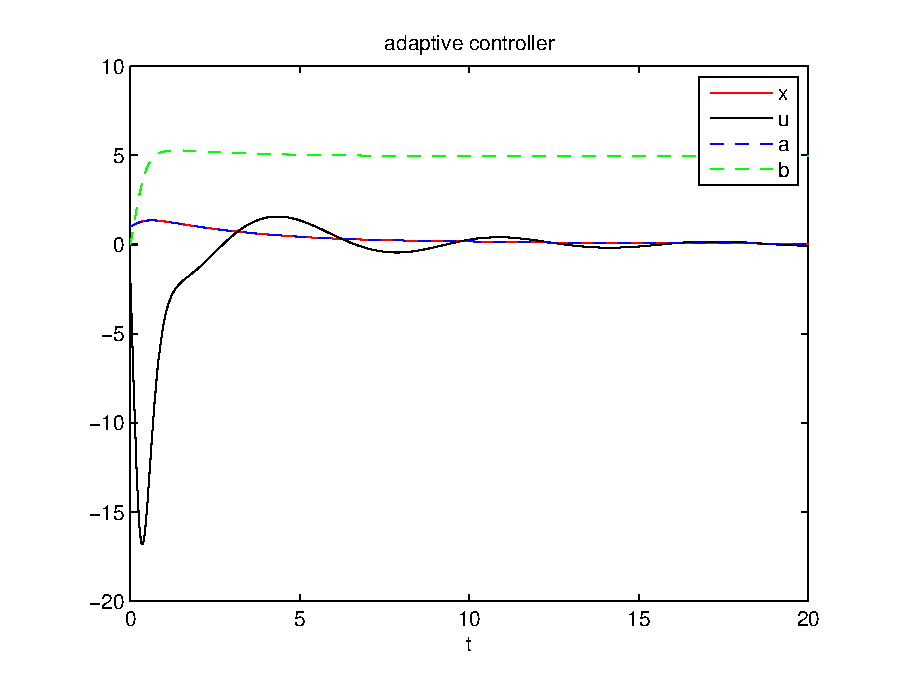
\includegraphics[width=0.7\textwidth]{figs/adap_controller.eps}% 1\linewidth
%  \centering
  \caption{simulation results of the adaptive control.}
  \label{adap_control}
\end{figure}

\indent For simulation, we set the system model to $m(x,\theta)=a(x^2+1)+b$ and $f(x,\dot x,t,\theta)=a\dot x+bx\sin(t)$, with $a$ and $b$ being the unknown parameters. Matlab ode45 function is used to simulate the system and test the performance of the adaptive controller. The initial condition of the system is set to $x_0=1$, $\dot x_0=1$, $\hat a_0=0$ and $\hat b_0=0$. The control gain and the parameter update gain are set to $k=1$ and $\Gamma=I$, respectively. The simulation results are shown in Figure \ref{adap_control}.

\subsection{Sliding Mode Controller}

\indent Assuming that $\left|\frac12\dot m(x,\theta)r+\alpha\dot xm(x,\theta)+f(x,\dot x,t,\theta)\right|\le\rho(x,\dot x,t)$ and $m(x,\theta)>0$, design the sliding mode controller as
\begin{equation}
u=-kr-\rho sgn(r).
\end{equation}

\indent Choose the Lyapunov function as
\begin{equation}
V=\frac12m(x,\theta)r^2.
\label{v}
\end{equation}
Taking the derivative of (\ref{v}) yields
\begin{equation}
\begin{aligned}
\dot V&=\frac12\dot m(x,\theta)r^2+m(x,\theta)r\dot r\\
&=\frac12 m(x,\theta)r^2+r\left[f(x,\dot x,t,\theta)+u+m(x,\theta)\alpha\dot x\right]\\
&=\left[\frac12\dot m(x,\theta)r+f(x,\dot x,r,\theta)+m(x,\theta)\alpha\dot x\right]r+r\left[-kr-\rho \cdot sgn(r)\right]\\
&\le \rho |r|+r\left[-kr-\rho \cdot sgn(r)\right]\\
&=-kr^2\le 0.
\end{aligned}
\end{equation}

\indent Since $V\ge 0$ and $\dot V \le 0$, $V\in L_\infty$. Therefore $r\in L_\infty$, $x\in L_\infty$, $\dot x\in L_\infty$ and $\dot r\in L_\infty$. According to Lemma 15, $kr^2\to 0$, so $x\to 0$.

\begin{figure}
  \centering
  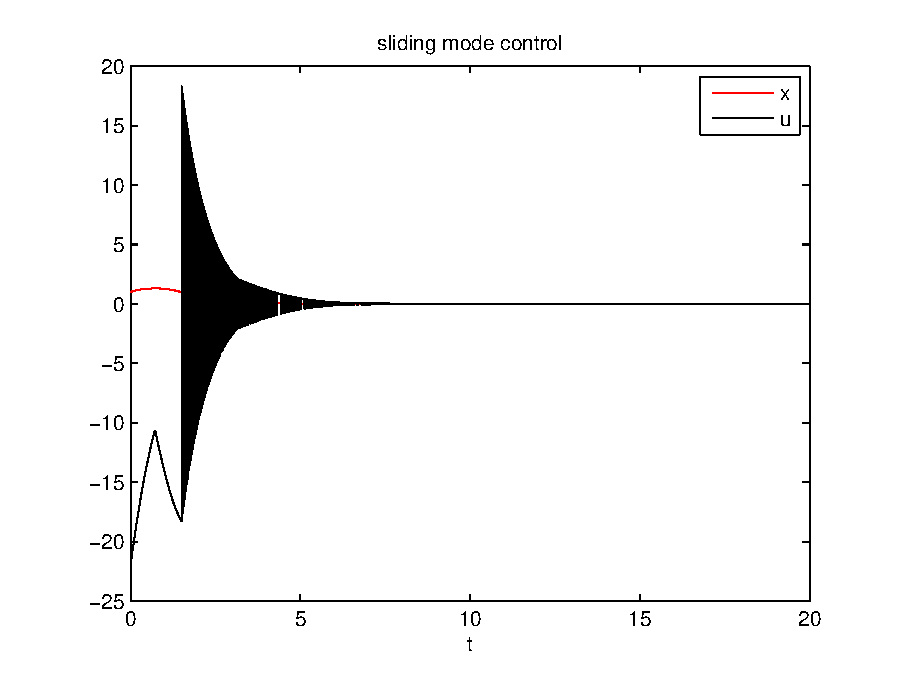
\includegraphics[width=0.7\textwidth]{figs/sliding_mode_control.eps}% 1\linewidth
%  \centering
  \caption{simulation results of the sliding mode control.}
  \label{sliding_mode}
\end{figure}

\indent For the simulation of the sliding mode controller, we use exactly the same system model and control parameters as the ones in the adaptive control. First, the bounding function $\rho(x,\dot x,t)$ needs to be determined. Assuming that $a\le \bar a$ and $b\le\bar b$, 
\begin{equation}
\begin{aligned}
&\left|\frac12\dot m(x,\theta)r+\alpha\dot xm(x,\theta)+f(x,\dot x,t,\theta)\right|\\
&\le \left| axr+\alpha\dot x(ax^2+a+b)+a\dot x+bx\sin(t) \right|\\
&\le \bar a|xr|+[\bar ax^2+2a+b]\cdot |\dot x|+\bar b |x \sin (t)|.
\end{aligned}
\end{equation}

Let $\rho(x,\dot x,t)=\bar a|xr|+[\bar ax^2+2a+b]\cdot |\dot x|+\bar b |x \sin (t)|$, and the sliding mode control can be simulated. The results are shown in Figure \ref{sliding_mode}. Note that though the control error goes to zero, the control input will oscillates around zero.


\subsection{Robust Controller}

\subsubsection{High Gain Feedback Robust Control}

\indent Assuming that $\left|\frac12\dot m(x,\theta)r+\alpha\dot xm(x,\theta)+f(x,\dot x,t,\theta)\right|\le\rho(x,\dot x,t)$ and $m(x,\theta)>0$, design the high gain feedback robust controller as
\begin{equation}
u=-kr-k_n\rho^2 r.
\end{equation}

\indent Choose the Lyapunov function as
\begin{equation}
V=\frac12m(x,\theta)r^2.
\label{v_highgain}
\end{equation}
Taking the derivative of (\ref{v}) yields
\begin{equation}
\begin{aligned}
\dot V&=\frac12\dot m(x,\theta)r^2+m(x,\theta)r\dot r\\
&=\frac12 m(x,\theta)r^2+r\left[f(x,\dot x,t,\theta)+u+m(x,\theta)\alpha\dot x\right]\\
&=\left[\frac12\dot m(x,\theta)r+f(x,\dot x,r,\theta)+m(x,\theta)\alpha\dot x\right]r+r\left[-kr-k_n\rho^2 r\right]\\
&\le \rho |r|+r\left[-kr-k_n\rho^2 r\right]\\
&=-kr^2+(\rho|r|-k_n\rho^2r^2)\\
&\le -kr^2+\frac{1}{k_n}\\
&= -2kV+\frac{1}{k_n}.
\end{aligned}
\label{dotv}
\end{equation}
Lemma 9 can be applied to (\ref{dotv}) to obtain the upper bound of $V$ as follows
\begin{equation}
V\le V_0e^{-2kt}+\frac{1}{2kk_n}\left(1-e^{-2kt}\right).
\label{vle}
\end{equation}
As a result, $V\in L_\infty$ satisfies
\begin{equation}
\lim_{t\to\infty}V\le \frac{1}{2kk_n}.
\end{equation}
From (\ref{v_highgain}) we know that $r,m\in L_\infty$. Therefore $x\in L_\infty$, $\dot x\in L_\infty$, $u\in L_\infty$ and $\dot r\in L_\infty$. All the signals in the closed-loop operation are bounded.

\indent From (\ref{v_highgain}) and (\ref{vle}), the $r$ satisfies
\begin{equation}
|r|\le \sqrt{r^2_0e^{-2kt}+\frac{1}{kk_n}\left(1-e^{-2kt}\right)}.
\label{vle}
\end{equation}
thus
\begin{equation}
\lim_{t\to\infty}|r|\le\sqrt{\frac{1}{kk_n}}
\end{equation}
Hence, $r$ is GUUB. Therefore, $x,\dot x$ are both GUUB.

\begin{figure}
  \centering
  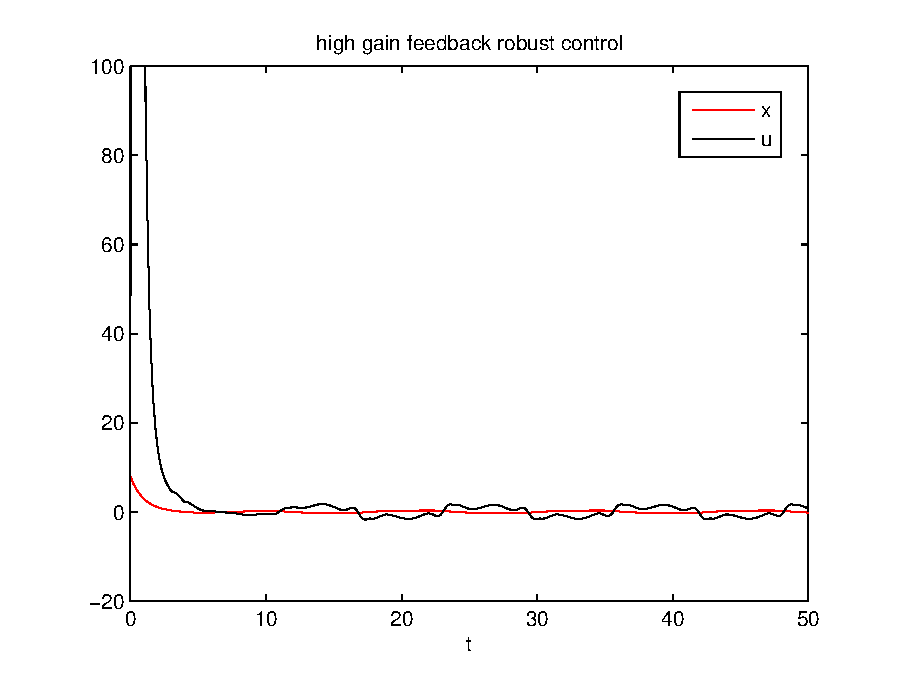
\includegraphics[width=0.7\textwidth]{figs/high_gain.eps}% 1\linewidth
%  \centering
  \caption{simulation results of the high gain feedback robust control.}
  \label{high_gain}
\end{figure}

\indent The experimental setup of the high gain feedback robust control is the same as the sliding mode control. The simulation results are shown in Figure \ref{high_gain}. From the results we can see that there is no oscillation phenomenon in the high gain feedback control. However, the control gain need to be fairly large to drive the control error to zero.

\subsubsection{High Frequency Feedback Robust Control}

\indent Assuming that $\left|\frac12\dot m(x,\theta)r+\alpha\dot xm(x,\theta)+f(x,\dot x,t,\theta)\right|\le\rho(x,\dot x,t)$ and $m(x,\theta)>0$, design the high frequency feedback robust controller as
\begin{equation}
u=-kr-\frac{\rho^2r}{\rho|r|+\varepsilon}.
\end{equation}

\indent Choose the Lyapunov function as
\begin{equation}
V=\frac12m(x,\theta)r^2.
\label{v_highf}
\end{equation}
Taking the derivative of (\ref{v}) yields
\begin{equation}
\begin{aligned}
\dot V&=\frac12\dot m(x,\theta)r^2+m(x,\theta)r\dot r\\
&=\frac12 m(x,\theta)r^2+r\left[f(x,\dot x,t,\theta)+u+m(x,\theta)\alpha\dot x\right]\\
&=\left[\frac12\dot m(x,\theta)r+f(x,\dot x,r,\theta)+m(x,\theta)\alpha\dot x\right]r+r\left[-kr-\frac{\rho^2r}{\rho|r|+\varepsilon}\right]\\
&\le \rho|r|+r\left[-kr-\frac{\rho^2r}{\rho|r|+\varepsilon}\right]\\
&= -kr^2+\frac{\rho|r|\varepsilon}{\rho|r|+\varepsilon}\\
&\le -kr^2+\varepsilon\\
&=-2kV+\varepsilon.
\end{aligned}
\label{dotvf}
\end{equation}
Lemma 9 can be applied to (\ref{dotvf}) to obtain the upper bound of $V$ as follows
\begin{equation}
V\le V_0e^{-2kt}+\frac{\varepsilon}{2k}\left(1-e^{-2kt}\right).
\label{vlef}
\end{equation}
As a result, $V\in L_\infty$ satisfies
\begin{equation}
\lim_{t\to\infty}V\le \frac{\varepsilon}{2k}.
\end{equation}
From (\ref{v_highgain}) we know that $r,m\in L_\infty$. Therefore $x\in L_\infty$, $\dot x\in L_\infty$, $u\in L_\infty$ and $\dot r\in L_\infty$. All the signals in the closed-loop operation are bounded.

\indent From (\ref{v_highf}) and (\ref{vlef}), the $r$ satisfies
\begin{equation}
|r|\le \sqrt{r^2_0e^{-2kt}+\frac{\varepsilon}{k}\left(1-e^{-2kt}\right)}.
\label{vlef}
\end{equation}
thus
\begin{equation}
\lim_{t\to\infty}|r|\le\sqrt{\frac{\varepsilon}{k}}
\end{equation}
Hence, $r$ is GUUB. Therefore, $x,\dot x$ are both GUUB.

\begin{figure}
  \centering
  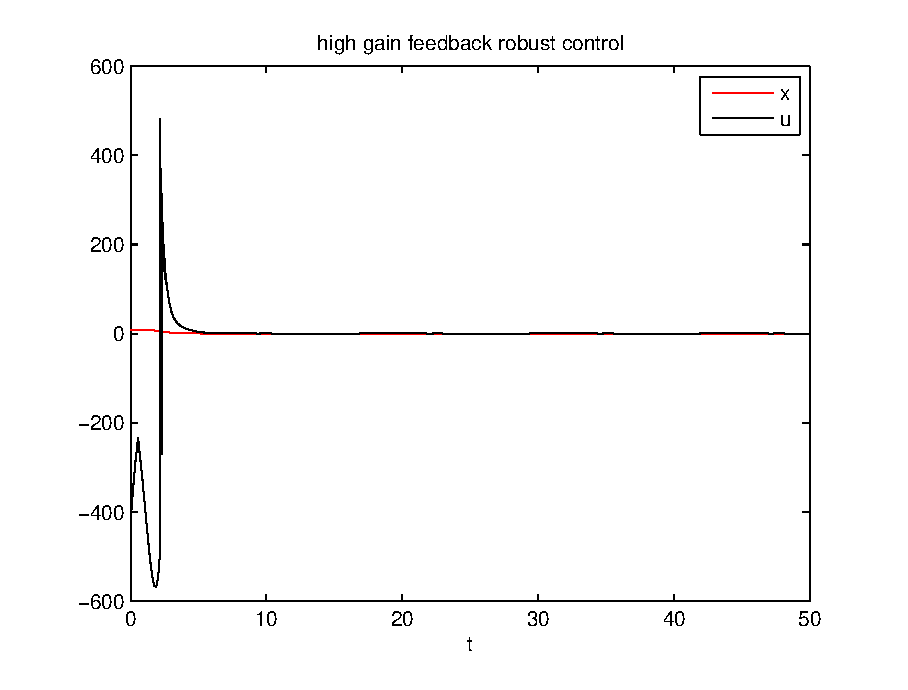
\includegraphics[width=0.7\textwidth]{figs/high_freq.eps}% 1\linewidth
%  \centering
  \caption{simulation results of the high frequency feedback robust control.}
  \label{high_freq}
\end{figure}

\indent The experimental setup is the same as the high gain feedback robust control. The parameter $\varepsilon$ is set to 0.1. The simulation results are shown in Figure \ref{high_freq}. The control gain is not as large as the one in the high gain feedback robust control. In Figure \ref{high_gain}, we manually bound the y axis for the sake of visualization.

\end{document} 